\chapter{Compile-Time PLT Redex Representation}

This chapter describes how PyPltRedex represents constructs of PLT Redex described in Chapter 02 and establishes notation to be used throughout the report. Additionally, forms that are not part of PLT Redex are also introduced.

\section{Define Language}

This form defines languages.

\begin{lstlisting}
define-language ::= (define-language language-name non-terminal-definition ... +)
non-terminal-definition ::= (non-terminal-name ::= pattern ... +)
\end{lstlisting}


Compile-time representation of `define-language` follows the grammar defined above closely. More specifically, 

\begin{itemize}
\item
`DefineLanguage(name, ntdef)` represents `define-language` form. 
\item
`NtDefinition(sym, patterns)` represents `non-terminal-definition` inside `define-language`
\end{itemize}

\section{Metafunctions}
Supported subset of `define-metafunction` grammar is as follows:

\begin{lstlisting}
(define-metafunction language-name
  metafunction-contract
  metafunction-case ...)

metafunction-contract =	id : pattern-sequence ... -> pattern 
metafunction-case =  [(name pattern ...) term] 
\end{lstlisting}

A metafunction is a function on terms. The define-metafunction form builds a metafunction according to the pattern and right-hand-side expressions. The first argument indicates the language used to resolve non-terminals in the pattern expressions. Each of the rhs-expressions is implicitly wrapped in term. (TODO rewrite this)

TODO example metafunction definition.

\section{Reduction Relation}

\begin{lstlisting}
reduction-relation ::= (reduction-relation language domain reduction-case ...)
reduction-case     ::= (-> pattern term reduction-case-name)
domain ::= #:domain pattern
\end{lstlisting}

This form had to be modified. Example of this modification can be seen in Figure ??? below. Since PyPltRedex does not interpret Racket in any capacity, introducing `(define id expr)` form (which evaluates `expr` and assigns it to `id`) would have resulted in additional unnecessary complexity; more specifically, keeping track of forms that are not allowed to be used with `define` form such as `define-language`. Thus, `define` and `reduction-relation` were collapsed into a single form `define-reduction-relation`. In addition, use of `define` form to define reduction-relations seems to be inconsistent with respect to `define-language` and `define-metafunction` forms.


`domain` optional parameter provides contract for reduction relation. When `reduction-relation` is applied to a term, it has to satisfy the contract; that is the term must match provided pattern otherwise it is an error. Similarly, after applying reduction relation to the term, resulting term(s) also have to sastisfy said contract; that is each term has to match the pattern provided by `domain`.

\section{Pattern Language}

This section describes subset of PltRedex's pattern specification language supported by \texttt{PyPltRedex}. Grammar for the pattern language can be seen below, in EBNF notation. 

\begin{lstlisting}
pattern = number 
        | integer 
		| real 
		| natural 
		| string 
		| boolean 
		| variable-not-otherwise-mentioned 
		| hole 
		| symbol
        | (in-hole pattern pattern)
        | (pattern-sequence *) 
pattern-sequence : pattern 
                 | pattern ...  # literal ellipsis
\end{lstlisting}

\begin{itemize}
\item
\textit{number} pattern matches any number.

\item
\textit{integer} matches any exact integer. 

\item
\textit{real} matches any real number.

\item
\textit{natural} matches any natural number; that is any non-negative integer.

\item
\textit{string} matches any string.

\item
\textit{boolean} matches any boolean - \texttt{\#t} or \texttt{\#f}.
\item
\textit{variable-not-otherwise-mentioned} matches any symbol that is not used as a literal in language definition. For example, if language definition contains pattern \texttt{(+ number number)} \textit{variable-not-otherwise-mentioned} will not match symbol \texttt{+}.

\item
\textit{hole} matches \texttt{hole} term exactly.

\item
\textit{symbol} matches any symbol except if its value coincides with non-terminal symbol in language definition.
\end{itemize}

All pattern above except \textit{hole} can be suffixed with underscore and identifier (for example, \textit{number\_1}) to create binding to matched term.

\begin{itemize}
\item
\textit{(in-hole pattern pattern)} traverses the term trying to match the second pattern; upon successful match the term matching the second pattern is replaced with term `hole` and then the first pattern is matched. First pattern must match exactly one hole.

\item
\textit{pattern-sequence} pattern matches a term list, where each pattern-sequence element matches an element of the list. Each individual pattern within the sequence can be suffixed with \texttt{...} (literal ellipsis) and that will match zero or more terms matching the pattern.
\end{itemize}

If patterns in the pattern-sequence are suffixed with the same identifier (e.g. \texttt{(number\_1 number\_1)})), then the match is contrained to terms that are equal. That means term \texttt{(1 1)} matches the pattern but \texttt{(1 2)} does not. For patterns in \textit{define-language} constraint checking is not performed. PltRedex provides other constraint checks but they will not be considered.

\section{Compile-time Representation of Patterns}

Throughout the report the following notation will be used to represent actual Python classes used to implement the pattern language. Actual Python source code can be seen on page (TODO-appendix reference). 

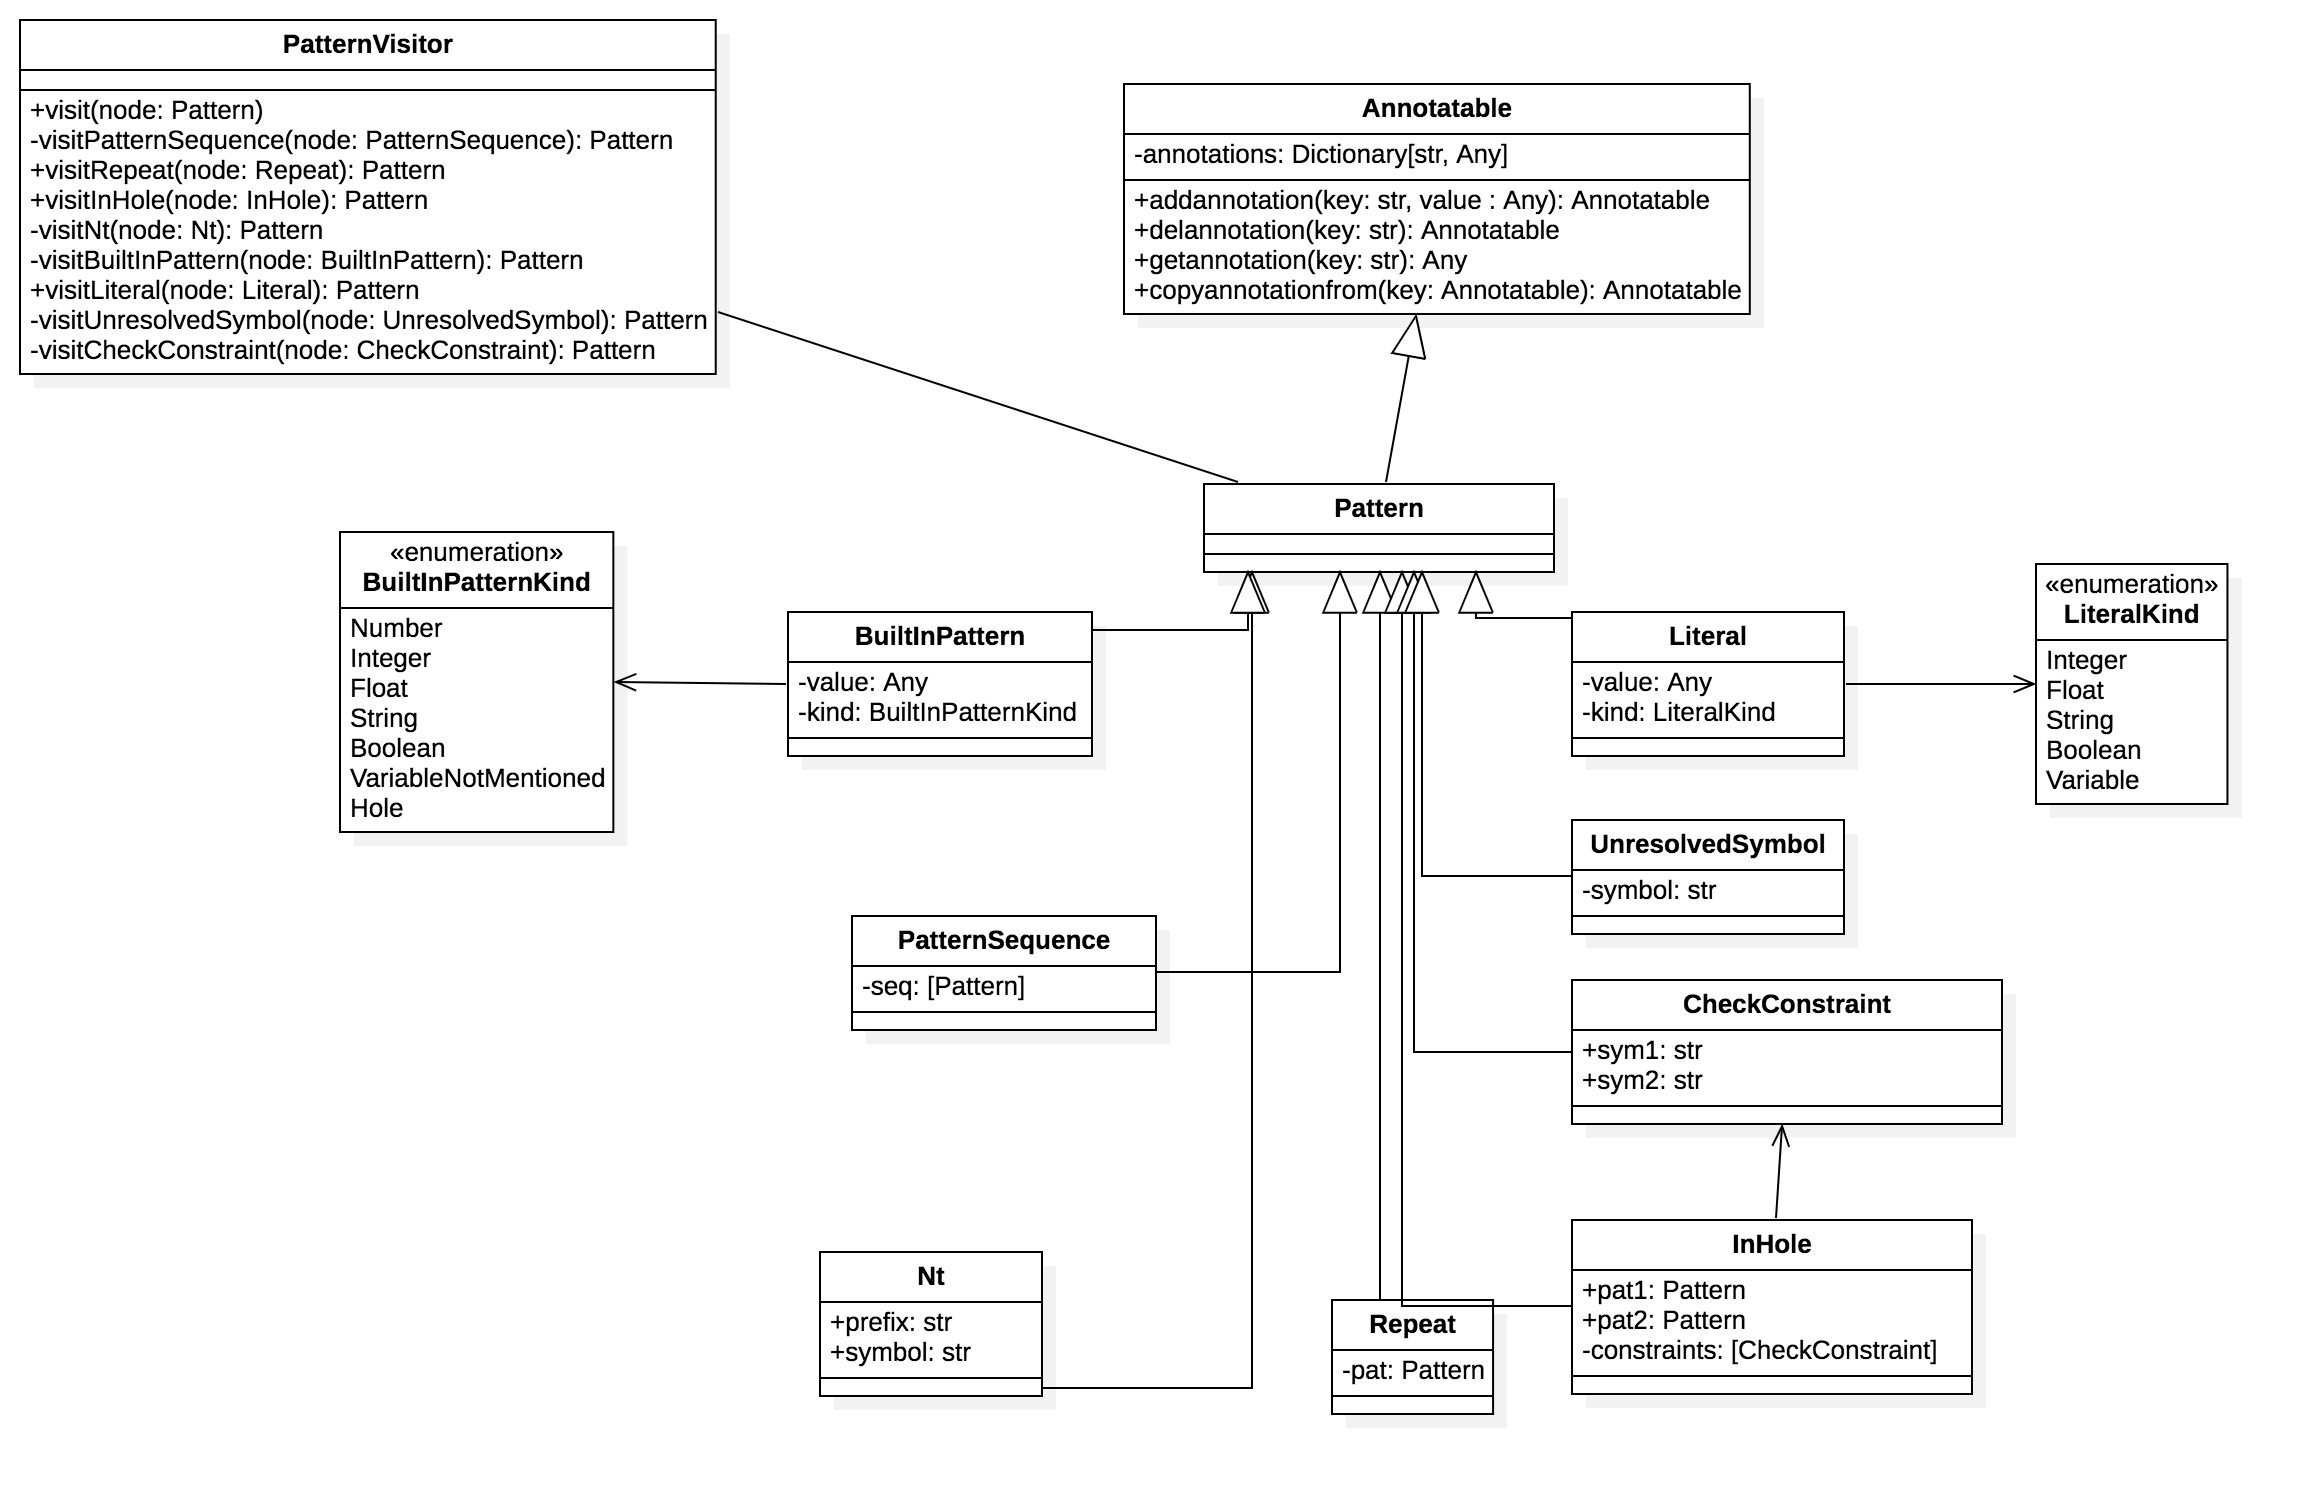
\includegraphics[scale=0.175]{class-diagram-pattern.png}


\begin{itemize}
\item
\PatternSequence represents `pattern-sequence` clause of the pattern language and may contain zero or more child patterns $p_i$.

\item 
\Repeat represents pattern $p$ under ellipsis.

\item 
\Nt represents non-terminal. $nt$ is a non-terminal symbol, while $s$ is the symbol used for binding terms. For example, given pattern \texttt{e\_1} $s$ is \texttt{e\_1} and $nt$ is \texttt{e}.
\item
\BuiltInPattern represents various built-in patterns such as \texttt{number} or \texttt{string}. $t$ is the tag and must be picked from set $T$. $s$ is the symbol used for binding terms.

\item
\InHolePattern represents \texttt{in-hole} pattern, $p_1$ and $p_2$ must be patterns.

\item 
\LiteralPattern represents a literal values in patterns. Since literal values can be of many types, a tag $l$ must be provided from set $T$. $v$ is actual literal value.

\item 
\UnresolvedSymbol used to represent symbols that are initially unknown to be non-terminal or literal, $s$ is the symbol.

\item
\CheckConstraint is used for equality checking of terms. Terms bound to $s_1$ and $s_2$ are checked for equality.

\end{itemize}

TODO UML diagram

\section{Terms}

The compile-time representation of terms differs greatly from the runtime representation described previously. The reason for this is the necessity to handle ellipses; or, more specifically substitution of pattern variables under ellipses - \texttt{PltRedex} handles this dynamically and erroneous ellipses aren't detected until term creation time.
It is desirable to handle ellipsis depth checking of pattern variables at compile time to be able to provide compile time error messages. Doing this allows for the complete elimination of ellipses from the runtime (with variable \texttt{...} being a reserved symbol that throws an Exception). In addition, this also allows for detection of metafunction applications statically.

The grammar for terms can be found below. To differentiate between runtime terms, the compile-time representation of terms will be called \textbf{term-templates}.

\begin{lstlisting}
term-template = pattern-variable 
              | (term-sequence *)
              |,(functionname term*) 
              |(in-hole term term)
              | hole
	          | integer
	          | float
	          | string
	          | boolean 
term-sequence = term
              | term ... ; literal ellipsis
              | ,@(function term *)
              | ,@(function term *) ...; literal ellipsis FIXME is this the case?
\end{lstlisting}

\begin{itemize}
\item 
\lstinline{pattern-variable} represents pattern variables.
\item
\lstinline{,(functionname term*)} calls user-implemented RPython function with zero or more terms as arguments.
\item
\lstinline{,@(functionname term*)} calls user-implemented RPython function with zero or more terms as arguments that must return a list. Contents of the returned list are then inserted into term-sequence at that position. 
\item
\lstinline{(in-hole term term)} locates \lstinline{hole} in the first term and replaces it with the second term.
\item
\lstinline{hole} represents term \lstinline{hole}
\item
\lstinline{integer} represents any literal integer.
\item
\lstinline{float} represents any literal floating point number.
\item
\lstinline{string}  represents any literal string.
\item
\lstinline{boolean}  represents any literal boolean.
\item
\lstinline{term-sequence} represents a list of term.  Each individual term within the sequencecan be suffixed with ...(literal ellipsis) indicating ellipsis depth of the term-template.
\end{itemize}

\section{Compile-time Representation of Term-Templates}

Throughout the report the following notation will be used to represent actual Python classes used to implement the term-templates. Actual Python source code can be seen on page (TODO-appendix reference). 


\begin{lstlisting}
type TermLiteralKind = Variable
                     | Integer 
                     | Float 
                     | String
                     | Boolean
                     | Hole

type PyCallMode = Normal | Splice  

type TermTemplate = PatternSequence($t_1$: TermTemplate, ..., $t_n$: TermTemplate)
                  | Repeat($t$: TermTemplate)
                  | InHole($t_1$: TermTemplate, $t_2$: TermTemplate)
                  | PythonCall($m$: PyCallMode, $t_1$: TermTemplate, ..., $t_n$: TermTemplate)
                  | Literal($l$: TermLiteralKind, $v$: Any)
                  | PatternVariable($s$: string)
                  | UnresolvedSymbol($s$: string)
\end{lstlisting}

\begin{itemize}
\item \TermSequence represents term sequences and may contain zero or more child term-templates $t_i$.
\item \TermRepeat represents term sequence under ellipsis.
\item \TermInHole represents \lstinline{in-hole} term template
\item \PythonCall represents \lstinline{,(functionname term*)} and \lstinline{,@(functionname term*)} term-template. Variable $m$ is used to indicate which case it actually is - $m$ is set to \lstinline{Normal} if it is the first, otherwise \lstinline{Splice}.
\item \TermLiteral - represents any literal in term-template. It is initialized with appropriate tag.
\item \PatternVariable - represents all pattern variables.
\item \TermUnresolvedSymbol - represents unresolved symbols. Initially it is unknown if some symbol is pattern-variable or a literal.
\end{itemize}


\section{Additional Testing Forms}

PyPltRedex provides several additional forms with testing functionality. The goal is to run individual components of PyPltRedex, such as pattern matcher and term generator, and compare the results against expected ones. These additional forms are \texttt{redex-match-assert-equal}, \texttt{term-let-assert-equal} and \texttt{apply-reduction-relation-assert-equal}. They are defined in the following manner (and this notation will be used throughout the report):

\begin{lstlisting}
type MatchAssignment = MatchAssignment($s$: string, $t$: Term)
type Match = Match($a_1$: MatchAssignment, ..., $a_n$: MatchAssignment)
type PA = PatternVariableAssignment($v$: string, $i$: natural, $t$: Term)
type TopLevelForm = RedexMatchAssertEqual($l$: string, $p$: Pattern, $t$: Term, $m_1$: Match, ..., $m_n$: Match)
                  | TermLetAssertEqual($a_1$: PA, ..., $a_n$: PA, $t$: Term, $e$: Term)
                  | ApplyReductionRelationAssertEqual($r$: string, $t$: Term, $e_1$: Term, ..., $e_n$: Term)
                  | TopLevelForm
\end{lstlisting}

These forms provide the following functionalities:

\begin{itemize}
\item 
\texttt{redex-match-assert-equal}: Given a term, it is matched against a pattern that may contain non-terminal symbols from \texttt{language}. It compares the resulting list of matches against the expected list. The order in which the expected matches appear in the list is important. An Exception is raised under the following conditions:
	\begin{enumerate}
	\item Lengths of both lists do not match.
	\item Given two matches from both lists at position $i$, $m_i^{expected} \neq m_i^{actual}$, with equality operation defined in TODO.
	\end{enumerate}
	This form is based on \texttt{redex-match} form provided by PLT Redex.


\item 
\texttt{term-let-assert-equal}: Given a list of pattern-variable assignments, it replaces all pattern-variables in term-template with terms bound to pattern-variables and then asserts that the resulting term is equal to the expected one.  While this form is based on the \texttt{term-let} form provided by PltRedex, the way assignments are specified is different. In PltRedex, assignment is `(pattern term)` (i.e. term is matched against the pattern and terms bound by the match are then used to replace pattern-variables), whereas PyPltRedex bypasses matching step. `integer` in assignment represents ellipsis depth of the pattern-variable and assumes that related term is well-formed regarding ellipsis depth. That is, `(n 1 (term (1 2 3)))` is valid but `(n 1 (term ((1) (2) (3))))` is not.

\item 
\texttt{apply-reduction-relation-assert-equal} This form takes a term-template, applies reduction-relation (assuming reduction-relation is defined and thus `reduction-relation-name` is valid), and ensures that a list of terms after reduction is equal to a predefined list of terms. An Exception is raised under the following conditions:

	\begin{enumerate}
	\item Lengths of both lists do not match.
	\item Given two terms from both lists at position $i$, $t_i^{expected} \neq t_i^{actual}$, with equality operation defined in TODO.
	\end{enumerate}
\end{itemize}
This form is based on \texttt{apply-reduction-relation} from provided by PLT Redex.

\section read-from-stdin-and-apply-reduction-relation

Form ReadFromStdinAndApplyReductionRelation(reductionname: string, mfapply: string?) is rather self-explanatory - it reads a string from standard input or file, parses it into a term using logic outlined in Section TODO, and applies reduction-relation \texttt{reductionname}. Optionally, one can provide metafunction with name \texttt{mfapply} to apply to the parsed term. This allows to separate specification of "code" from everything else that is required to evaluate the "code" (such as model of the heap/stack, etc) TODO.



